\subsection{階層型NNによる学習}
\subsubsection{最適なパラメータを探すためのアプローチ}
指定された条件下において学習が効率良く行われるパラメータの組み合わせを探
すため、最初は1つの値づつ、大まかな値から設定して調べ、徐々に値の細かくしていくことでパラメータを調整した。

\subsubsection{実行結果}

\begin{table}[htb]
 \begin{center}
  \caption{階層型NNによるExOR問題の学習に要した回数}
  \label{table:level2}
  \begin{tabular}[htb]{r|l} \hline
   シード値 & 収束した回数 \\ \hline \hline
   1000 &  15622\\ \hline
   2000 &  110\\ \hline
   3000 &  100000\\ \hline
   4000 &  100000\\ \hline
   5000 &  100000\\ \hline
   6000 &  17180\\ \hline
   7000 &  27237\\ \hline
   8000 &  4394\\ \hline
   9000 &  6665\\ \hline
   10000 &  100000\\ \hline \hline
   10試行の平均値 &  47130.8\\ \hline
  \end{tabular}
 \end{center}
\end{table}

\begin{figure}[h]
 \begin{center}
  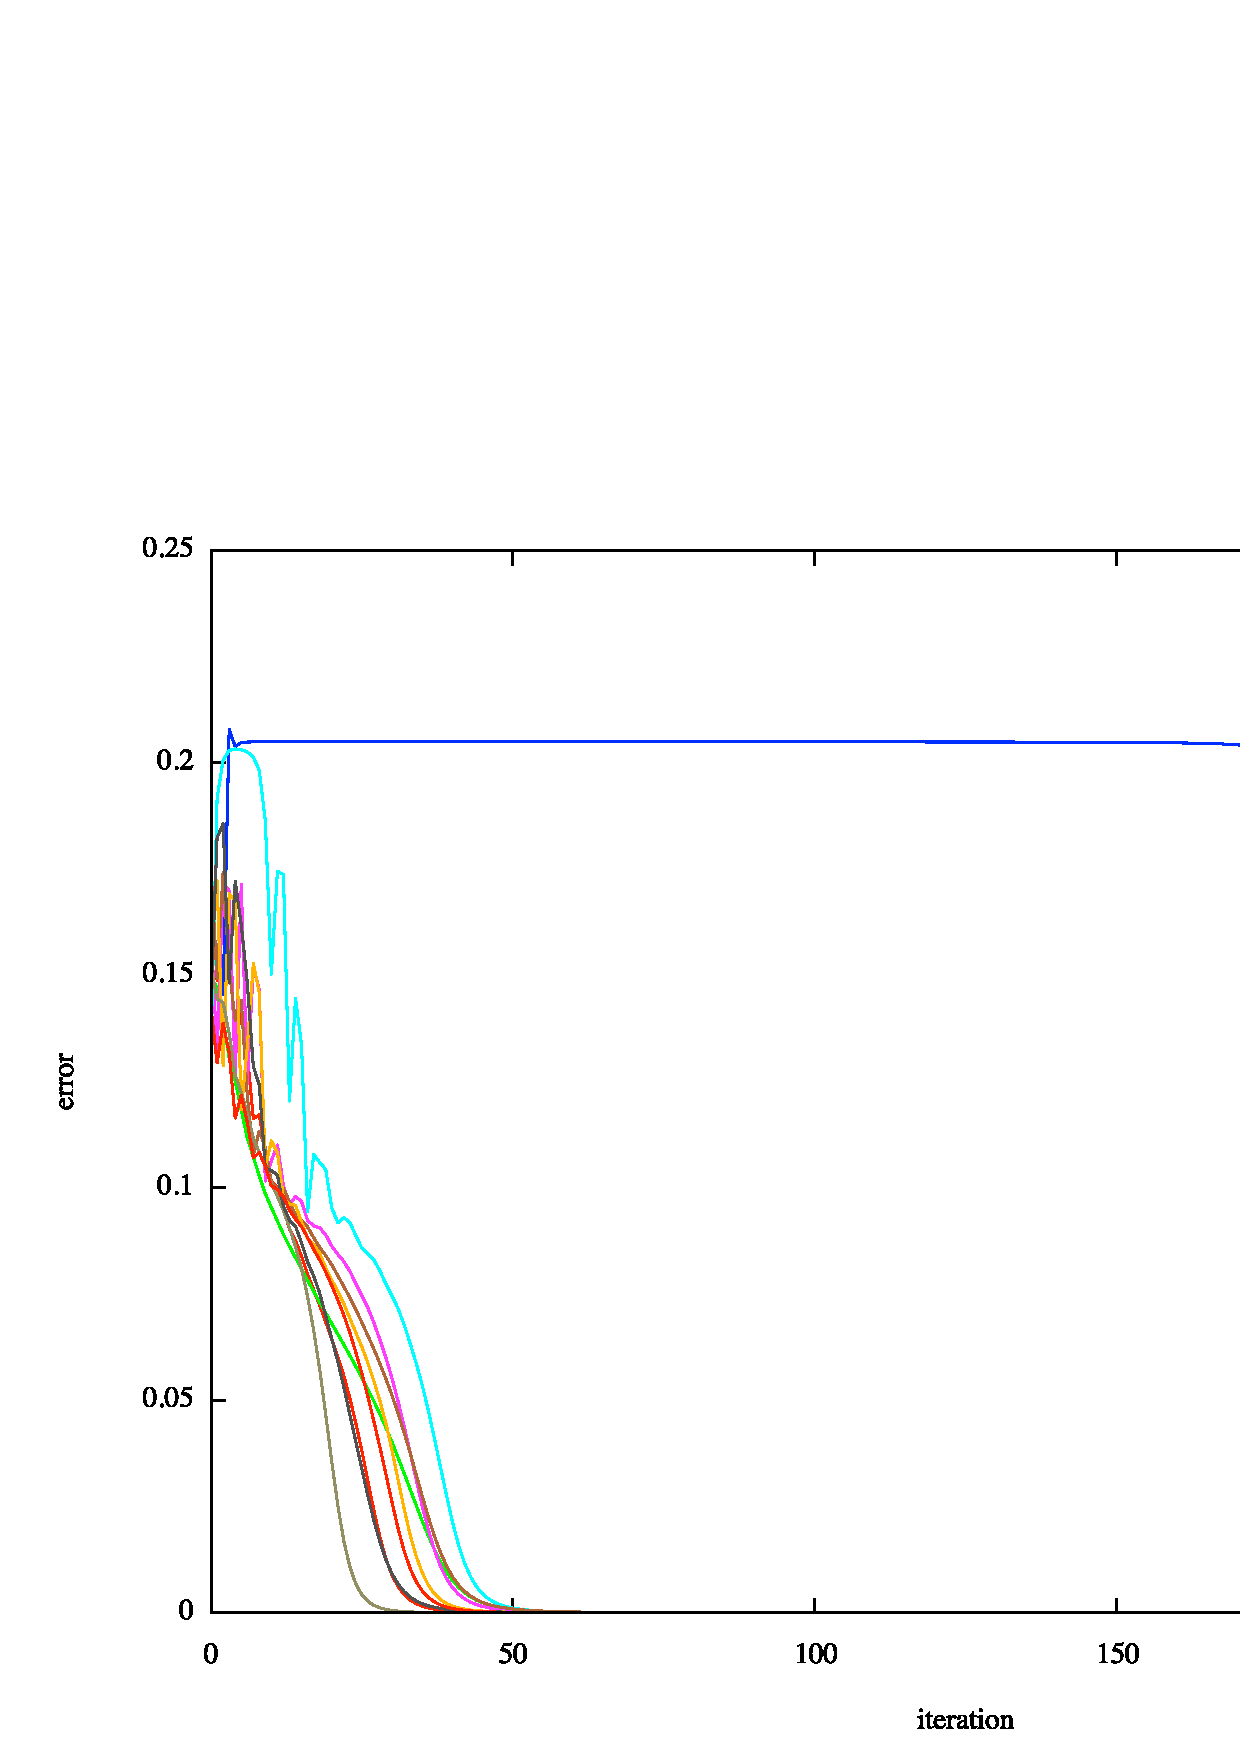
\includegraphics[width=10.0cm]{level2/exor_ave.pdf}
  \caption{重みを更新する様子(平均値)}
  \label{fig:level2}
 \end{center}
\end{figure}


\subsubsection{考察}
alphaやETAは高い値の方が誤差が低い結果となったが、HIDDENに関しては必ずしも荘ではなく、16という比較的低い数字で誤差が小さくなったので、中間層のユニットは多ければ多い程良いというわけではないと考えられる。
